\documentclass[a4paper, 12pt]{article}
\usepackage[utf8]{inputenc}
\usepackage[T1]{fontenc}
\usepackage[french]{babel}
\usepackage{graphicx}
\usepackage{amsmath}
\usepackage{hyperref}
\usepackage{lmodern}
\usepackage{moreverb}
\usepackage{multicol}


\usepackage[a4paper,left=2cm,right=2cm,top=2cm,bottom=2cm]{geometry}

\pagestyle{headings}
\pagestyle{plain}

\usepackage{listings}


\setcounter{secnumdepth}{4}
\setcounter{tocdepth}{4}
\makeatletter


\makeatother

\makeatletter
\def\toclevel@subsubsubsection{4}
\def\toclevel@paragraph{5}
\def\toclevel@subparagraph{6}
\makeatother

\setlength{\parindent}{0cm}
\setlength{\parskip}{1ex plus 0.5ex minus 0.2ex}
\newcommand{\hsp}{\hspace{20pt}}
\newcommand{\HRule}{\rule{\linewidth}{0.5mm}}

\begin{document}

\begin{titlepage}
  \begin{sffamily}
  \begin{center}

   
    \textsc{\LARGE }\\[2cm]

    \textsc{\Large Compte rendu de Réunion}\\[1.5cm]
    \textsc{\Medium Rédigé par Idriss BENGUEZZOU}

    % Title
    \HRule \\[0.4cm]
    { \huge  \textsc{StellaStone} \\
    \textsc{\Large By Novus}\\ [0.4cm] }
	
    \HRule \\[2cm]
    \textsc {Idriss BENGUEZZOU\\Ghilas MEZIANE}
 \begin{figure}
     \centering
    
\includegraphics[scale=0.2]{logoUJM.png}
     \label{fig:ujm_logo}
 \end{figure}

    \vfill

    % Bottom of the page
    {\large {} 27/01/2023}

  \end{center}
  \end{sffamily}
\end{titlepage}


\newpage

\section{Réunion du Vendredi 27/01}

Comme prévue lors de la précédente réunion, la réunion de cette semaine a eu lieu le vendredi 27 janvier 2023, en distanciel sur le créneau horaire 18h00 - 20h00, sur discord. Celle-ci s’est tenue avec la présence de tous les membres du groupe.
\\\\
\textbf{Ordre du jour}
\begin{itemize}
    \item Échange sur l'avancée et sur les difficultés rencontrées
    \item Mise en place de conventions de clean code.
\end{itemize}


\subsection{Tour de table}

Le langage C\# a été adopté facilement car il est similaire au langage Java. En effet, C\# possède des similitudes en terme de structure de code, des concepts et des bibliothèques d'outils. Les deux langages utilisent le modèle orienté objets et partagent des fonctionnalités pour les bases de données.

Idriss a déclaré que la mise en place des effets visuels (VFX) a été assez facile pour lui grâce à la documentation détaillée et aux nombreux tutoriels disponibles en ligne. Cependant, il a également mentionné qu'il a eu du mal à comprendre les concepts plus avancés tels que les shaders et les particules.

Ghilas a mentionné qu'il avait déjà une expérience préalable avec Cinema 4D pour la modélisation d'objets en 3 dimensions, mais il a déclaré que la réalisation d'objets en 3 dimensions a été un peu plus difficile dans Unity car l'interface lui semblait trop compliquée pour réaliser des formes complexes.

Nous avons trouvé une solution pour pallier à ce problème, notamment en utilisant des modèles prédéfinis (libres de droits) téléchargeables sur Internet.
Un des principaux problèmes rencontrés avec les modèles téléchargés sur internet a été la nécessité d'installer un logiciel tiers pour permettre à Unity d'importer ces modèles. Par exemple, pour les fichiers .blend nous avons été contraints d'installer blender pour convertir le fichier .blend en fichier (fbx) pouvant être lu par Unity. 
Suite à l'installation de Blender, nous avons modélisé la fusée présente sur notre maquette. 

 \begin{figure}[!h]
    \centering
    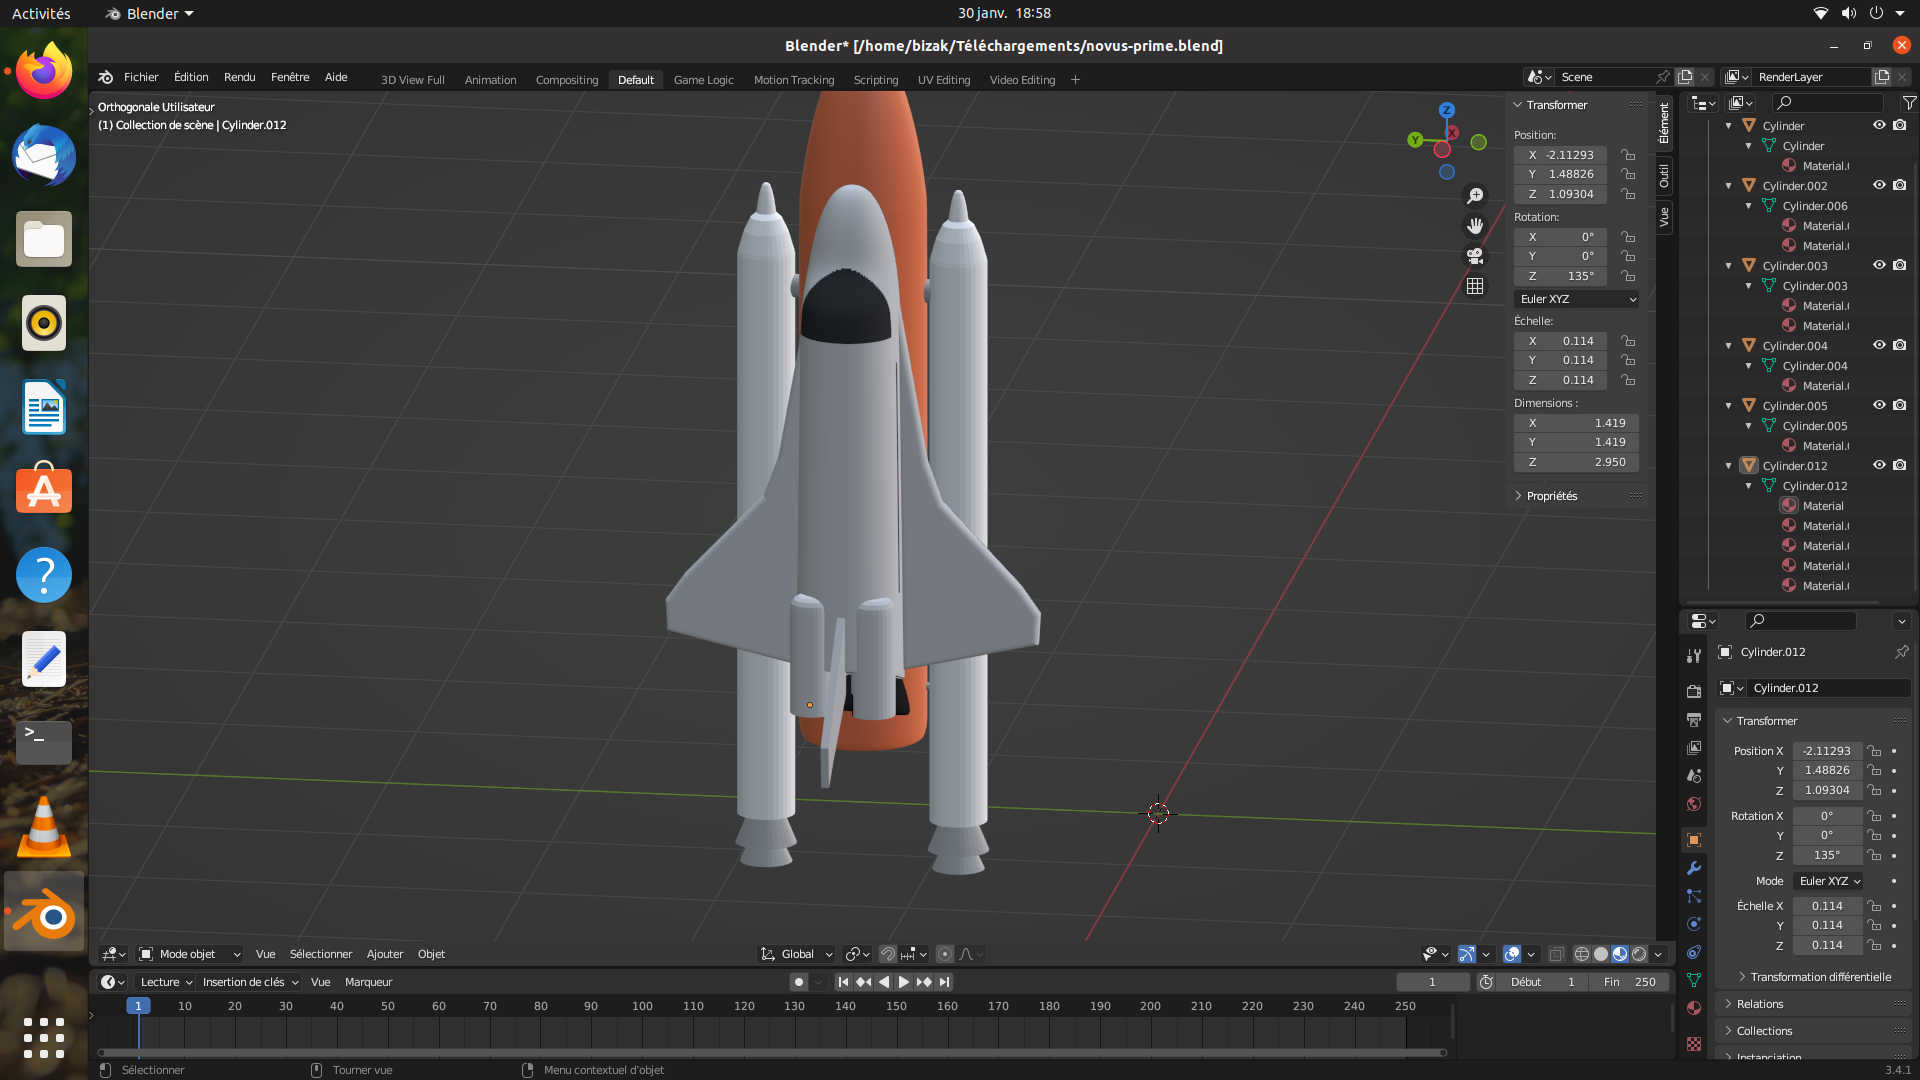
\includegraphics[scale=0.2]{fuseeBlender.png}
    \label{fig:Le_planning}
    \caption{Modélisation 3D de la fusée}
\end{figure}

\newpage

De même, Idriss a déclaré avoir commencé à découvrir les différentes méthodes pour animer les objets dans la scène. Ceci se fait via des scripts rédigés en C\#. Par exemple comme première étape, il a pu modéliser un cube posé sur un plan, pilotable grâce aux flèches directionnelles. 

\begin{figure}[!h]
    \centering
    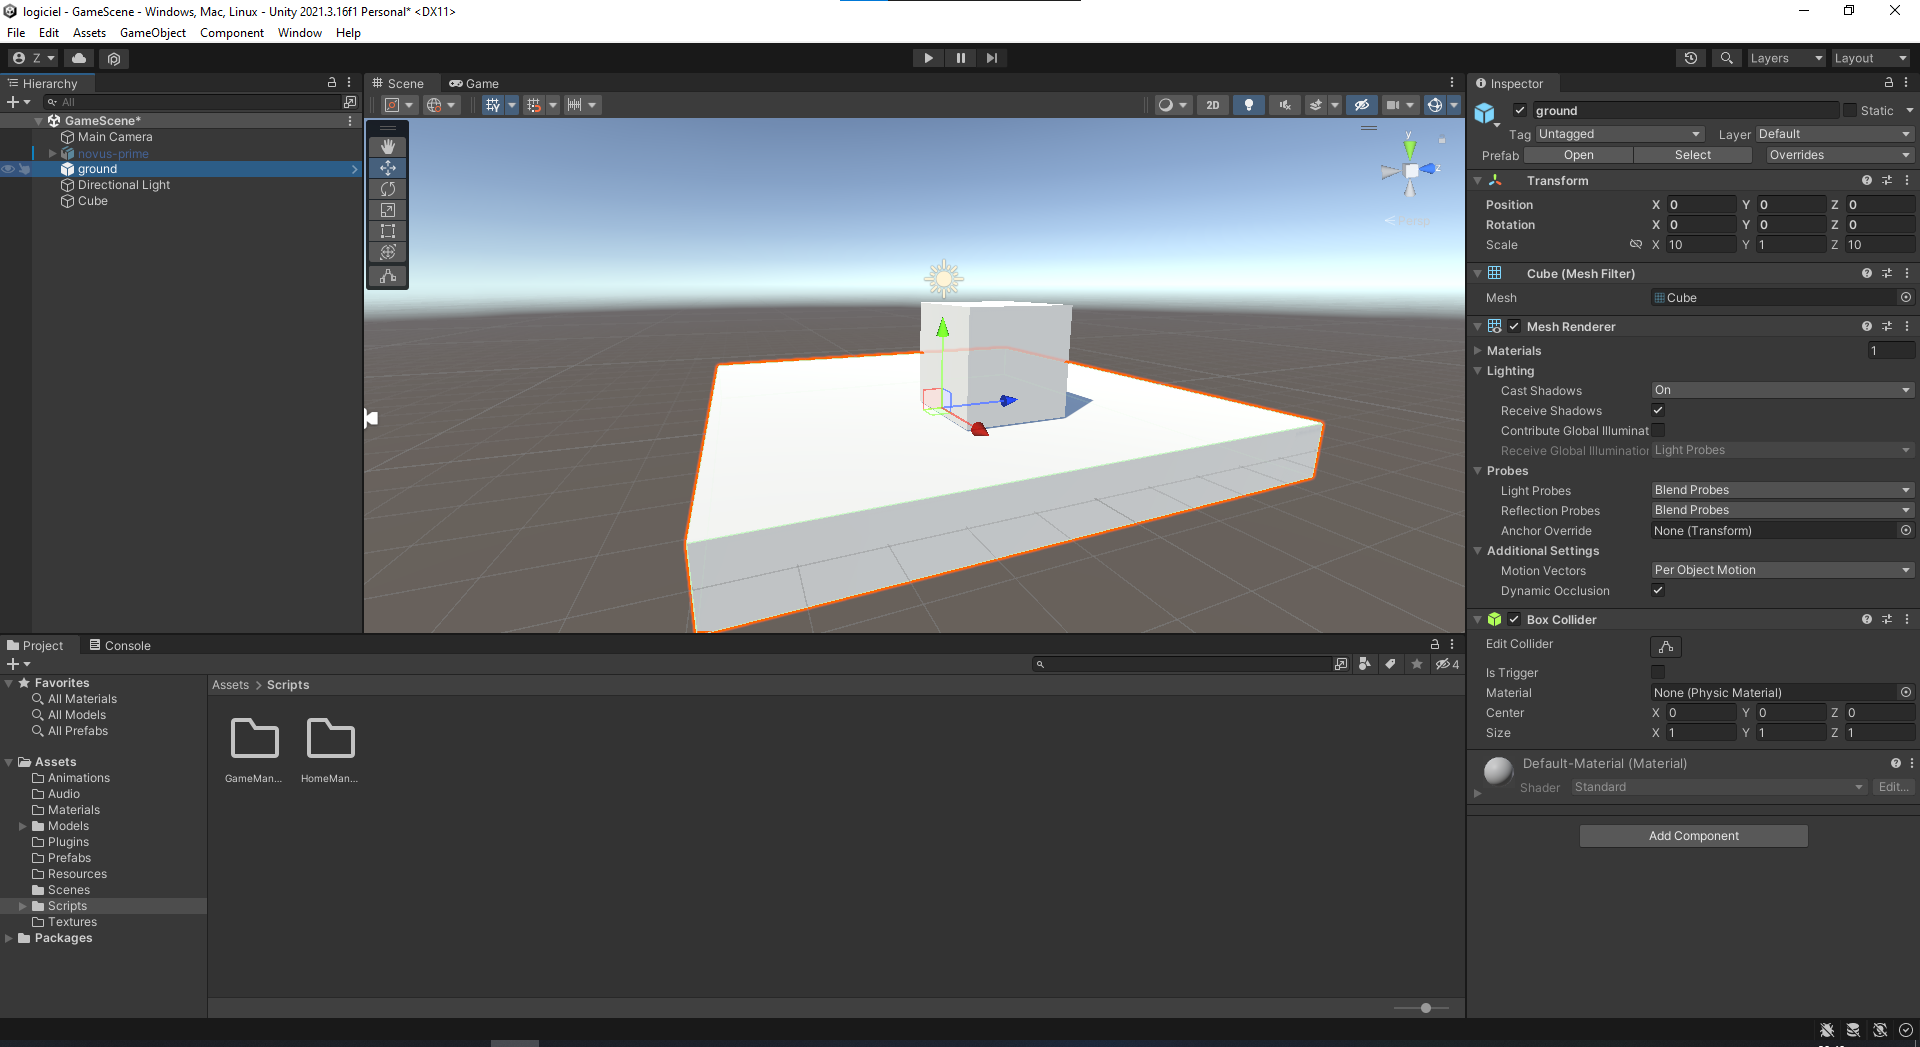
\includegraphics[scale=0.27]{cube.png}
    \label{fig:Le_planning}
    \caption{L'objet pilotable}
\end{figure}

\newpage

\section{Architecture}

Lors de cette réunion, nous avons également déterminé l'architecture des fichiers du projet. En recherchant les architectures les plus courantes utilisées pour la réalisation de jeux vidéos en 3 dimensions, nous avons opté pour une structure simple et facile à utiliser, organisant les différents éléments du projet dans des dossiers dédiés. 

La structure comprend un dossier "Scènes" qui contient les fichiers définissant la structure de la scène 3D, le dossier "Scripts" qui contient les fichiers de code en C\# qui définissent le comportement des objets dans la scène, le dossier "Prefabs" qui contient les préfabriqués, qui sont des objets prédéfinis qui peuvent être réutilisés dans plusieurs scènes, le dossier "Materiaux" qui contient les matériaux utilisés pour définir l'apparence des objets dans la scène, les "Textures" qui contient les textures utilisées pour donner plus de détails aux objets, le dossier "Audio" qui contient les sons utilisés dans la scène, le dossier "Models" qui contient les fichiers de modèle 3D utilisés pour les objets dans la scène, le dossier "Animations" qui contient les animations pour les objets dans la scène et le dossier "VFX" qui contient les fichiers pour les effets visuels.

Cette structure solide nous permettra de travailler efficacement sur le projet en maintenant une bonne organisation.
\\
\begin{lstlisting}[language=Bash]
- Assets/
    - Scenes/
    - Scripts/
    - Prefabs/
    - Materials/
    - Textures/
    - Audio/
    - Models/
    - Animations/
    - Plugins/
    - Resources/
    - VFX
- Library/
- ProjectSettings/
\end{lstlisting}

\section{Planification du travail de la semaine à venir}

Suite à cette première semaine de découverte de l'environnement Unity, Ghilas MEZIANE et Idriss BENGUEZZOU ont constaté que la modélisation et la mise en place des éléments graphiques prendra beaucoup de temps compte tenu de la quantité d'objet a modéliser. 

L'objectif pour la prochaine semaine sera d'initialiser la scène graphique pour la mission spatiale en commençant par la mise en place de la zone de lancement de la fusée. Ainsi que de la mise en place de l'interface d'accueil.

Lors de la semaine écoulée nous n'avons pas eu l'occasion d'écrire beaucoup de code. Nous préférons donc nous familiariser un peu plus avec le langage C\# avant de mettre en place les conventions de Clean code qui nous accompagneront durant ce semestre.

L'objet de la prochaine réunion, qui se tiendra le 03/02/2023, sera de d'observer l'avancement du projet en général.

\end{document}